\documentclass[12pt]{book}
\usepackage{diffyqssetupUB}

\begin{document}

%extra material {Linearization, critical points, and equilibria}

%\sectionnewpage
\subsection{Vector fields of 2D systems with Python}\label{Vector_fields_of_2D_systems_with_Python:subsection}

The \emph{resources306} module provides a function \emph{fieldplot} 
to plot the vector field of the two-dimensional autonomous system of ODEs \eqref{eq:nlinautn2}.
It works just like \emph{fieldplotlinear} except that 
{\color{blue} instead of a matrix,}
it takes a {\color{blue}pair of} 
{\color{red}general (nonlinear)}
function{\color{blue}s} of two variables.
You supply a Python function that takes the pair $(x,y)$ 
{\color{red}(can be a tuple, a list, or an array)}
{\color{teal}BH distracting detail}
and returns the pair $(f(x,y),g(x,y))$.
{\color{blue}You also give}{\color{red}along with} the desired ranges for the horizontal and vertical axes, followed by any desired graphical options.
In the example below we use \emph{fieldplot} to make a vector field plot for the system
\begin{equation} 
\begin{bmatrix} x \\ y \end{bmatrix} ' =
\begin{bmatrix} -y \cos(x+y-1) \\ x \cos(x-y+1) \end{bmatrix} .
\end{equation}


\begin{small}
\begin{verbatim}
from resources306 import *
def F(X):
    x,y = X
    return -y*cos(x+y-1), x*cos(x-y+1)
cos = np.cos
plt.figure(figsize=(10,10))
plt.subplot(111,aspect=1)  # optional: make scales same on the two axes
fieldplot(F,-2,5,-2.5,2.5,color='b',alpha=0.5)

\end{verbatim}
\end{small}

\parbox[c]{3.1in}{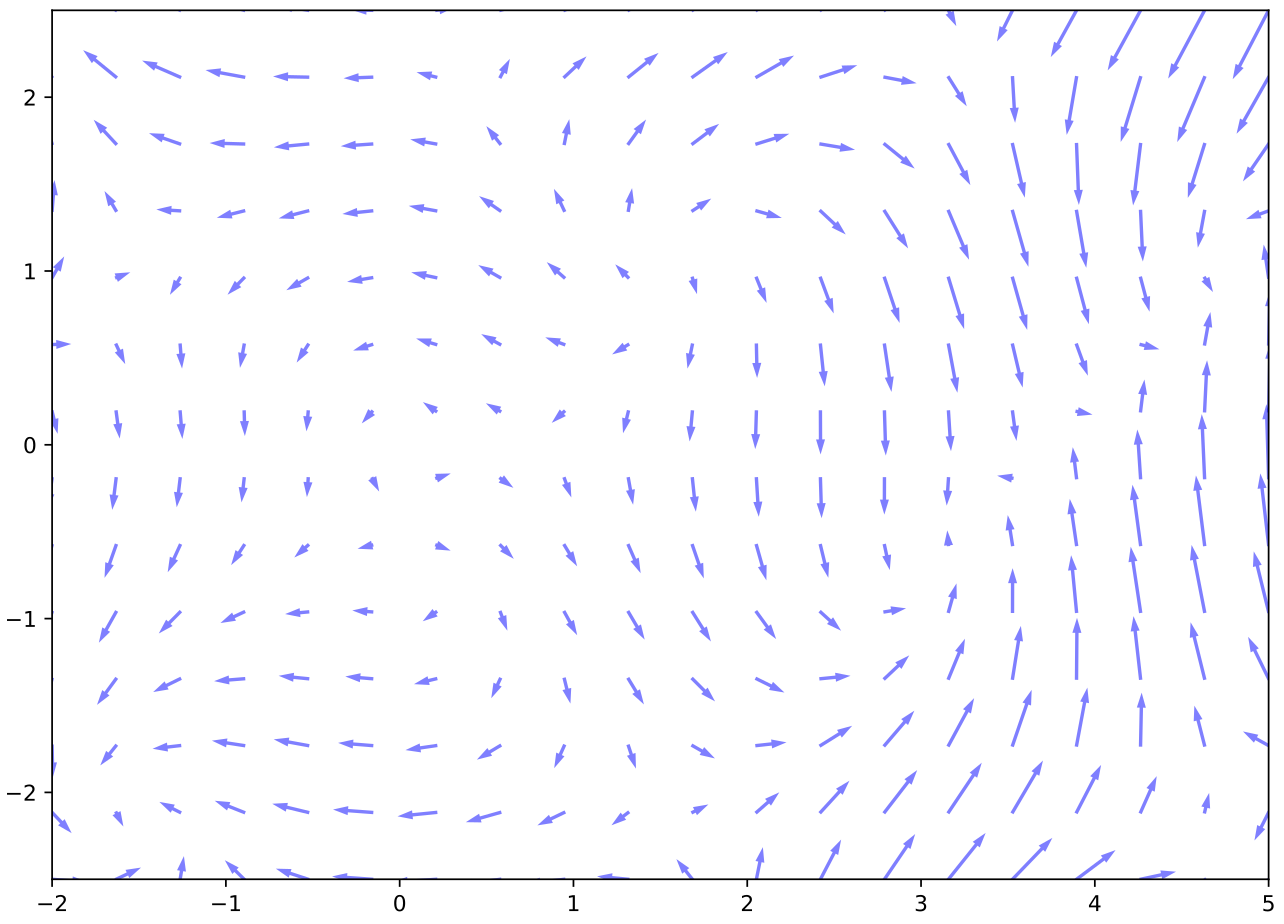
\includegraphics[width=5.5in]{additional_figures/Nonlinear_systems__fieldplot}}
\newpage

{\color{teal}BH plot too small- changed width from 3.0 to 5.0 to make larger}
{\color{red}
\noindent There is also a function \emph{phaseportrait} for computing and drawing solutions curves that we will
describe in the next Section [TODO: put in section ref]. 
}
{\color{teal}BH Time to remove TODOs its 20190730 already}


%extra material {Stability and classification of isolated critical points}

\sectionnewpage
\subsection{Phase portraits and equilibria with Python}

The \emph{resources306} module also provides a function \emph{phaseportrait} 
to numerically compute and plot solution curves of the two-dimensional autonomous system of ODEs \eqref{eq:nlinautn2}. 
This works just like \emph{phaseportraitlinear} described in \sectionref{Vector_fields_of_2D_systems_with_Python:subsection}, except
that instead of a matrix, 
you supply a Python function that takes the pair $(x,y)$ 
{\color{red}(can be a tuple, a list, or an array)}
{\color{teal}BH distracting detail}
and returns the pair $(f(x,y),g(x,y))$.
{\color{blue}This Python function can be the same one used with \emph{fieldplot}.}
{\color{red}
you supply a function that takes the pair $(x,y)$ (should work for a tuple, list, or array)
and returns the pair $(f(x,y),g(x,y))$.}
In the example below we use \emph{phaseportrait} to add some solution curves to the example from the previous
section. We also add dots to mark some equilibria. These are computed using \emph{fsolve}, which is imported by \emph{resources306} from the module
\emph{scipy.optimize}. You give \emph{fsolve} the function whose zero you want, and a rough guess at the location: \emph{fsolve} will
try to return an accurate approximation of the zero.
\begin{small}
\begin{verbatim}
from resources306 import *
def F(X):
    x,y = X
    return -y*cos(x+y-1), x*cos(x-y+1)
cos = np.cos
plt.figure(figsize=(10,10))
plt.subplot(111,aspect=1)  # optional: make scales same on the two axes

fieldplot(F,-2,5,-2.5,2.5,color='k',alpha=0.25)

phaseportrait(F, [(.25,0),(.25,.25),(.5,.5,-4,3),(-1,1),(-.5,.5),
                  (-1,-1),(2,1,-3,3),(1,1,-3,3)], color='k' )
x0,y0 = 0,0
x1,y1 = fsolve( F, (1,1) )
x2,y2 = fsolve( F, (3,-1) )
x3,y3 = fsolve( F, (0,4) )
x4,y4 = fsolve( F, (-2,-2) )
plt.plot(x0,y0,'ko', x1,y1,'ko', x2,y2,'ko', x3,y3,'ko', x4,y4,'ko')
\end{verbatim}
\end{small}

\parbox[c]{5.4in}{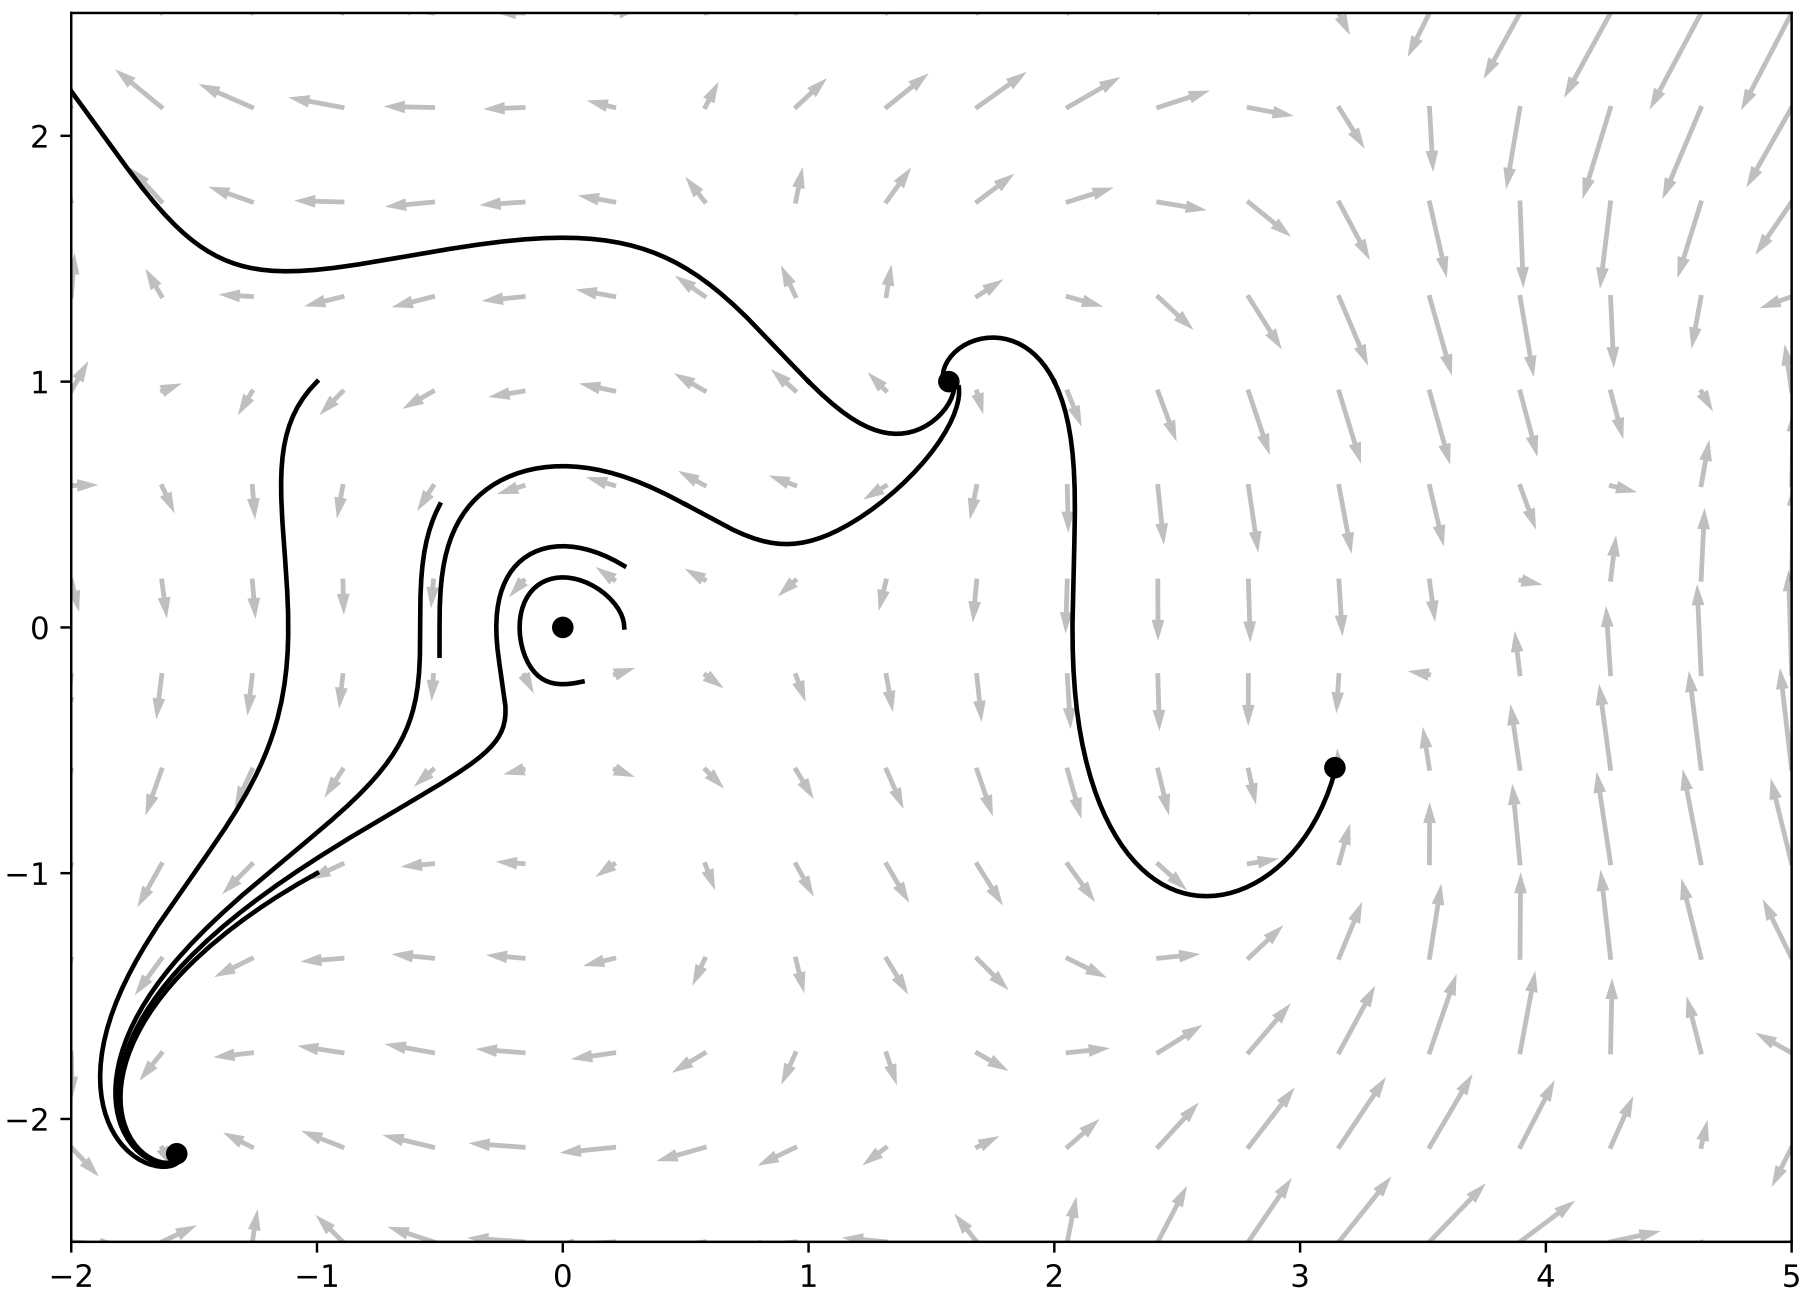
\includegraphics[width=4.8in]{additional_figures/Nonlinear_systems__phaseportrait_and_equilibria}}

{\color{teal}BH Tried cos=sp.cos and it didn't work, so cos from numpy}
{\color{teal}BH missing figures}
{\color{teal}BH graphic too small- changed includegraphics  width from 3.3in to 5.0in}

\end{document}

